\subsection{Sigma-Algebras and Measures}

% **Role:** modern integration and almost-everywhere analysis.
%
% Sigma-algebras, measures, outer measure, measurable sets, Borel/Lebesgue measure, null sets, regularity.

This subsection builds measurable sets before measurable integrals: set algebra, countable closure, Lebesgue measure, then measurable functions. Outer measure covers from outside; measurability splits test sets without losing measure.

\begin{definition} \label{def:measure-measurability-core-source-todo}\label{def:ring-sigma-ring-set-function} \hlt{Rings, $\sigma$-Rings, and Set Functions}\\
A \hlt{ring} of sets is closed under finite unions and relative complements.\\
A \hlt{$\sigma$-ring} is also closed under countable unions.\\
A \hlt{set function} on $\mathcal{A}$ is an extended-real map on $\mathcal{A}$ whose range does not contain both $+\infty$ and $-\infty$.\\
It is \hlt{additive} if $A\cap B=\emptyset$ implies $\phi(A\cup B)=\phi(A)+\phi(B)$.\\
It is \hlt{countably additive} if the same rule holds for pairwise disjoint countable unions: $\phi\left(\bigcup\limits_{n=1}^{\infty}A_n\right)=\sum\limits_{n=1}^{\infty}\phi(A_n)$.\\
\hlt{Structural Commentary}: Rings support finite additivity; $\sigma$-rings support countable limits.
\end{definition}

\begin{proposition} \label{prop:additive-set-function-basic-laws} \hlt{Basic Laws for Additive Set Functions}\\
Let $\phi$ be additive on a ring $\mathcal{A}$. Then:
\begin{enumerate}[label=(\roman*)]
\setlength{\itemsep}{0pt}
\item $\phi(\emptyset)=0$;
\item $\phi(A_1\cup\cdots\cup A_n)=\phi(A_1)+\cdots+\phi(A_n)$ for pairwise disjoint $A_i\in\mathcal{A}$;
\item $\phi(A\cup B)+\phi(A\cap B)=\phi(A)+\phi(B)$;
\item if $\phi$ is nonnegative and $A\subseteq B$, then $\phi(A)\leq\phi(B)$;
\item if $B\subseteq A$ and $\abs{\phi(B)}<+\infty$, then $\phi(A\setminus B)=\phi(A)-\phi(B)$.
\end{enumerate}
\begin{proof}
\begin{enumerate}[label=(\roman*)]
\setlength{\itemsep}{0pt}
\item Apply additivity to the empty disjoint union.
\item Induct on $n$, applying additivity to $(A_1\cup\cdots\cup A_{n-1})\cup A_n$.
\item By disjoint decompositions, $A\cup B=(A\setminus B)\cup(B\setminus A)\cup(A\cap B)$; $A=(A\setminus B)\cup(A\cap B)$; $B=(B\setminus A)\cup(A\cap B)$
\item If $A\subseteq B$, then $B=A\cup(B\setminus A)$ disjointly, so nonnegativity gives $\phi(A)\leq\phi(B)$.
\item If $B\subseteq A$, then $A=B\cup(A\setminus B)$ disjointly; since $\abs{\phi(B)}<+\infty$, subtract $\phi(B)$.
\end{enumerate}
\hlt{Structural Commentary}: Finite additivity plus disjoint decompositions controls all elementary identities.\\
\hlt{Key Insight}: Rewrite overlaps as disjoint pieces before applying $\phi$.
\end{proof}
\end{proposition}

\begin{theorem} \label{thm:continuity-from-below-set-functions} \hlt{Continuity from Below}\\
Suppose $\phi$ is countably additive on a ring $\mathcal{A}$.\\
If $A_1\subseteq A_2\subseteq A_3\subseteq\cdots$, and $A=\bigcup\limits_{n=1}^{\infty}A_n$ with all $A_n,A\in\mathcal{A}$, then $\phi(A_n)\to\phi(A)$.
\begin{proof}
Put $B_1=A_1$ and $B_n=A_n\setminus A_{n-1}$ for $n\geq2$. Then $B_n$ are pairwise disjoint, $A_n=B_1\cup\cdots\cup B_n$, and $A=\bigcup_nB_n$. Countable additivity turns $\phi(A_n)$ and $\phi(A)$ into partial sums and full sum of same series.\\
\hlt{Structural Commentary}: Increasing unions are disjoint tail decompositions in disguise.\\
\hlt{Key Insight}: Countable additivity converts set convergence into series convergence.
\end{proof}
\end{theorem}

\begin{definition} \label{def:elementary-sets-and-regular-set-functions} \hlt{Elementary Sets and Regularity in $\R^p$}\\
An \hlt{interval} in $\R^p$ is a coordinate box $a_i\leq x_i\leq b_i$, with endpoints optionally omitted; degenerate and empty cases are allowed. Define $m(I)\defeq\prod\limits_{i=1}^{p}(b_i-a_i)$ independent of endpoint inclusion.\\
A finite union of intervals is an \hlt{elementary set}; write $\mathcal{E}$ for all such sets.\\
If $A=I_1\cup\cdots\cup I_n$ is disjoint, set $m(A)\defeq m(I_1)+\cdots+m(I_n)$.\\
A nonnegative additive set function $\mu$ on $\mathcal{E}$ is \hlt{regular} if for every $A\in\mathcal{E}$ and $\varepsilon>0$ there are elementary sets $F\subseteq A\subseteq G$, with $F$ closed and $G$ open, such that $\mu(G)-\varepsilon\leq\mu(A)\leq\mu(F)+\varepsilon$. The source verifies that $\mathcal{E}$ is a ring, every elementary set has a disjoint interval decomposition, and $m$ is well defined, additive, and regular.
\end{definition}

\begin{perspective} \label{per:box-volume-and-linear-algebra} \hlt{Box Volume and Linear Algebra}\\
For a box $B=\prod_i(a_i,b_i)$ or $\prod_i[a_i,b_i]$, $m(B)=\prod_i(b_i-a_i)$, the diagonal case of determinant volume scaling.\\
Measure extends this product rule beyond boxes.\\
\hlt{Key Insight}: Lebesgue measure starts from determinant-style coordinate volume.
\end{perspective}

\begin{definition} \label{def:outer-measure-and-rudin-measurable-sets} \hlt{Outer Measure and $\mu$-Measurable Sets}\\
Let $\mu$ be additive, regular, nonnegative, and finite on $\mathcal{E}$.\\
For $E\subseteq\R^p$, define $\mu^\ast(E)\defeq\inf\sum\limits_{n=1}^{\infty}\mu(A_n)$, where infimum is over open elementary covers $E\subseteq\bigcup\limits_{n=1}^{\infty}A_n$.\\
For $A,B\subseteq\R^p$, set $A\triangle B\defeq(A\setminus B)\cup(B\setminus A)$ and $d_\mu(A,B)\defeq\mu^\ast(A\triangle B)$.\\
A set is \hlt{finitely $\mu$-measurable} if it is a $d_\mu$-limit of elementary sets.\\
It is \hlt{$\mu$-measurable} if it is a countable union of such sets; denote the classes by $\mathcal{M}_F(\mu)$ and $\mathcal{M}(\mu)$.
\end{definition}

\begin{definition} \label{def:tao-box-cover-outer-measure} \hlt{Box-Cover Outer Measure Model}\\
An \hlt{open box} in $\R^n$ is $B=\prod\limits_{i=1}^{n}(a_i,b_i)=\{(x_1,\ldots,x_n)\in\R^n:x_i\in(a_i,b_i) \ \forall i \}$, $b_i\geq a_i$, $\operatorname{vol}_n(B)\defeq\prod\limits_{i=1}^{n}(b_i-a_i)$.\\
For $\Omega\subseteq\R^n$, the \hlt{box-cover outer measure} is $m_n^\ast(\Omega)\defeq\inf\left\{\sum_{j\in J}\operatorname{vol}_n(B_j):(B_j)_{j\in J}\text{ covers }\Omega,\ J\text{ at most countable}\right\}$.\\
This is Definition \ref{def:outer-measure-and-rudin-measurable-sets} for Lebesgue box volume.
\end{definition}

\begin{figure}[H]
  \centering
  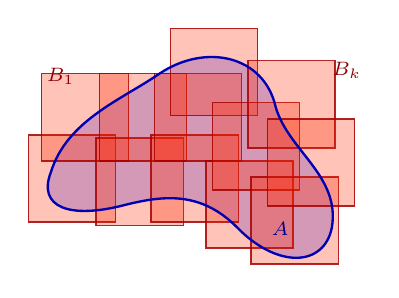
\begin{tikzpicture}[
  scale=0.82,
  every node/.style={font=\scriptsize},
  cover/.style={fill=red!70!orange, fill opacity=0.28, draw=red!65!black, draw opacity=0.85, line width=0.55pt},
  setfill/.style={fill=blue!65, fill opacity=0.34, draw=none},
  setoutline/.style={draw=blue!70!black, line width=0.85pt}
]
  \def\Ashape{%
    (-2.30,-0.42)
      .. controls (-2.05,0.38) and (-1.20,0.70) .. (-0.62,1.10)
      .. controls (0.10,1.58) and (1.00,1.38) .. (1.18,0.58)
      .. controls (1.38,-0.10) and (2.18,-0.48) .. (2.05,-1.28)
      .. controls (1.93,-1.90) and (1.20,-1.92) .. (0.58,-1.28)
      .. controls (0.02,-0.72) and (-0.55,-0.78) .. (-1.18,-0.94)
      .. controls (-2.00,-1.15) and (-2.52,-0.98) .. (-2.30,-0.42)
      -- cycle%
  }

  \path[setfill] \Ashape;

  \foreach \x/\y in {
    -2.65/-1.20,
    -2.45/-0.25,
    -1.60/-1.25,
    -1.55/-0.25,
    -0.75/-1.20,
    -0.70/-0.25,
    -0.45/0.45,
    0.10/-1.60,
    0.20/-0.70,
    0.75/-0.05,
    0.80/-1.85,
    1.05/-0.95
  }{
    \draw[cover] (\x,\y) rectangle ++(1.35,1.35);
  }

  \draw[setoutline] \Ashape;

  \node[blue!55!black] at (1.25,-1.30) {$A$};
  \node[red!55!black] at (-2.15,1.06) {$B_1$};
  \node[red!55!black] at (2.28,1.15) {$B_k$};
\end{tikzpicture}

  \caption{Cover $A\subseteq\bigcup_k B_k$ by squares; minimize $\sum_k\abs{B_k}$.}
  \label{fig:outer-measure-rectangle-cover}
\end{figure}

\begin{perspective} \label{per:outer-measure-geometric-box-covers} \hlt{Outer Measure as Outside Approximation}\\
Outer measure covers $A$ from outside; $d_\mu(A,B)=\mu^\ast(A\triangle B)$ measures closeness.\\
\hlt{Key Insight}: Countable subadditivity collects near-optimal covers.
\end{perspective}

\begin{method} \label{meth:lebesgue-measure-construction} \hlt{Lebesgue Measure Construction}\\
\begin{enumerate}[label=(\roman*)]
\setlength{\itemsep}{0pt}
\item \hlt{Cover from outside}\\
For $A\subseteq\R^n$, define $m_n^\ast(A)\defeq\inf\left\{\sum_{j\in J}\operatorname{vol}_n(B_j):(B_j)_{j\in J}\text{ covers }A,\ J\text{ at most countable}\right\}$.\\
This is defined for every set, but it is only countably subadditive in general.
\item \hlt{Keep the clean splitters}\\
Call $A$ measurable when every test set $X\subseteq\R^n$ splits additively: $m_n^\ast(X)=m_n^\ast(X\cap A)+m_n^\ast(X\cap A^c)$.\\
These measurable sets form a $\sigma$-algebra.
\item \hlt{Restrict the outer measure}\\
Define Lebesgue measure on measurable sets by $m(A)\defeq m_n^\ast(A)$.\\
On this restricted class, $m$ is countably additive.
\end{enumerate}
\hlt{Key Insight}: Outer measure sizes all sets; clean splitting restores additivity.
\end{method}

\begin{theorem} \label{thm:measure-measurability-main-source-todo}\label{thm:rudin-measure-extension} \hlt{Extension to a Measure}\\
Let $\mu$ be additive, regular, nonnegative, and finite on $\mathcal{E}$. Form $\mu^\ast$ from open elementary covers, set $d_\mu(A,B)=\mu^\ast(A\triangle B)$, and let $\mathcal{M}(\mu)$ be the countable unions of $d_\mu$-limits of elementary sets. Then:
\begin{enumerate}[label=(\roman*)]
\setlength{\itemsep}{0pt}
\item $\mu^\ast(A)=\mu(A)$ for $A\in\mathcal{E}$;
\item $\mu^\ast$ is countably subadditive;
\item $\mathcal{M}(\mu)$ is a $\sigma$-ring;
\item $\mu^\ast$ is countably additive on $\mathcal{M}(\mu)$.
\end{enumerate}
\begin{proof}
\begin{enumerate}[label=(\roman*)]
\setlength{\itemsep}{0pt}
\item Regularity gives $\mu^\ast(A)\leq\mu(A)$; compact closed approximants inside $A$ give the reverse inequality.
\item Cover each $E_n$ within $2^{-n}\varepsilon$ of $\mu^\ast(E_n)$; the combined cover proves subadditivity.
\item If $A_k\to A$, $B_k\to B$ in $d_\mu$, $A_k,B_k\in\mathcal{E}$, then $d_\mu(A_k\diamond B_k,A\diamond B)\leq d_\mu(A_k,A)+d_\mu(B_k,B)\to0$, $\diamond\in\{\cup,\cap,\setminus\}$.\\
Thus $\mathcal{M}_F(\mu)$ is a ring. If $A=\bigcup_kA_k$ with $A_k\in\mathcal{M}_F(\mu)$, then $A\setminus B=\bigcup_k(A_k\setminus B)$, so $\mathcal{M}(\mu)$ is a $\sigma$-ring.
\item For $A=\bigsqcup\limits_n A_n$, $A_n\in\mathcal{M}_F(\mu)$, subadditivity gives $\leq$,\\
while finite additivity gives $\mu^\ast(A)\geq\mu^\ast\left(\bigsqcup\limits_{n=1}^{N}A_n\right)=\sum\limits_{n=1}^{N}\mu^\ast(A_n)$.\\
Let $N\to\infty$, then decompose general disjoint families in $\mathcal{M}(\mu)$ into finite-measurable pieces.
\end{enumerate}
\hlt{Structural Commentary}: Elementary sets are completed under the distance measured by symmetric difference.\\
\hlt{Key Insight}: Approximate by elementary sets, prove identities there, then pass through $d_\mu(A,B)$.
\end{proof}
\end{theorem}

\begin{definition} \label{def:extended-and-lebesgue-measure} \hlt{Extended and Lebesgue Measure}\\
The \hlt{extended measure} is $\mu^\ast|_{\mathcal{M}(\mu)}$, denoted again by $\mu$.\\
For the elementary volume $m$, it is \hlt{Lebesgue measure} on $\R^p$.
\end{definition}

\begin{definition} \label{def:abstract-outer-measure-clean-division} \hlt{Abstract Outer Measure and Clean Division}\\
An \hlt{abstract outer measure} on $M$ is a monotone, countably subadditive function $\omega:2^M\to[0,+\infty]$ with $\omega(\emptyset)=0$.\\
A set $E\subseteq M$ is \hlt{$\omega$-measurable} if it cleanly splits every $X\subseteq M$: $\omega(X)=\omega(X\cap E)+\omega(X\cap E^c)$.\\
For Lebesgue outer measure, this is Caratheodory measurability.
\end{definition}

\begin{figure}[H]
  \centering
  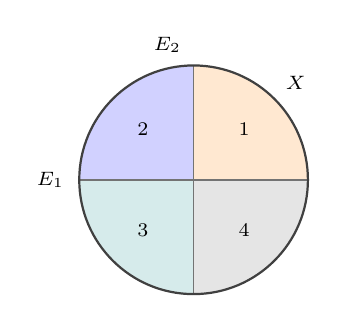
\begin{tikzpicture}[
  scale=0.88,
  every node/.style={font=\scriptsize},
  cut/.style={black!55, line width=0.65pt},
  boundary/.style={black!75, line width=0.8pt}
]
  \begin{scope}
    \clip (0,0) circle (1.65);
    \fill[orange!18] (0,0) rectangle (1.65,1.65);
    \fill[blue!18] (-1.65,0) rectangle (0,1.65);
    \fill[teal!16] (-1.65,-1.65) rectangle (0,0);
    \fill[black!10] (0,-1.65) rectangle (1.65,0);
    \draw[cut] (-1.65,0) -- (1.65,0);
    \draw[cut] (0,-1.65) -- (0,1.65);
  \end{scope}

  \draw[boundary] (0,0) circle (1.65);

  \node at (0.73,0.73) {$1$};
  \node at (-0.73,0.73) {$2$};
  \node at (-0.73,-0.73) {$3$};
  \node at (0.73,-0.73) {$4$};

  \node[above left=1pt] at (0,1.65) {$E_2$};
  \node[left=2pt] at (-1.65,0) {$E_1$};
  \node[above right=1pt] at (1.15,1.12) {$X$};
\end{tikzpicture}

  \caption{Two cuts split $X$ into four regions; $E_1\setminus E_2$ is region $2$.}
  \label{fig:measurable-difference-four-regions}
\end{figure}

\begin{theorem} \label{thm:caratheodory-measurable-sets-sigma-algebra} \hlt{Caratheodory Measurable Sets}\\
For any abstract outer measure $\omega$ on $M$, the $\omega$-measurable sets form a $\sigma$-algebra, and $\omega$ is countably additive there. Zero sets are measurable and may be added to or removed from measurable sets without changing measure.
\begin{proof}
If $\omega(Z)=0$, then for every $X\subseteq M$, $\omega(X)\leq\omega(X\cap Z)+\omega(X\cap Z^c)\leq0+\omega(X)$, so $Z$ is measurable; the same estimate handles changes by zero sets.\\
Complements are immediate, clean splitting is stable under differences, hence finite unions. If $E=\bigsqcup_iE_i$ with each $E_i$ measurable, finite additivity on partial unions and subadditivity give $\omega(X)=\sum\limits_{i=1}^{\infty}\omega(X\cap E_i)+\omega(X\cap E^c)$.\\
With $X=E$ this is countable additivity; for arbitrary $X$ it proves $E$ is measurable.\\
Disjointizing reduces general countable unions to this case.\\
\hlt{Structural Commentary}: Measurable sets preserve countable additivity.\\
\hlt{Key Insight}: Measurable cuts turn subadditivity into equality.
\end{proof}
\end{theorem}

\begin{lemma} \label{lem:open-sets-countable-unions-rational-boxes} \hlt{Open Sets Are Countable Unions of Rational Boxes}\\
Every open set $G\subseteq\R^n$ can be written as a finite or countable union of open boxes with rational endpoints.
\begin{proof}
The rational boxes are countable: each is determined by $2n$ rationals, and Corollary \ref{cor:rationals-countable} with Theorem \ref{thm:finite-tuples-over-countable-set-countable} makes finite rational tuples countable. Let $\Sigma$ be the rational boxes contained in $G$. Then $\bigcup_{B\in\Sigma}B\subseteq G$. If $\x\in G$, choose $r>0$ with $B_r(\x)\subseteq G$. By Corollary \ref{cor:rationals-and-irrationals-dense}, pick rationals $a_i,b_i$ satisfying $x_i-r/n<a_i<x_i<b_i<x_i+r/n$. Then $\x\in\prod_i(a_i,b_i)\subseteq B_r(\x)\subseteq G$, so $\x\in\bigcup_{B\in\Sigma}B$.\\
\hlt{Structural Commentary}: Rational boxes give a countable Euclidean base.\\
\hlt{Key Insight}: Openness supplies a ball; density of $\Q$ supplies rational box endpoints inside it.
\end{proof}
\end{lemma}

\begin{theorem} \label{thm:lebesgue-measure-basic-properties-checklist} \hlt{Lebesgue Measure Basic Properties}\\
Let $\mathcal{L}^n$ be the Lebesgue measurable subsets of $\R^n$, let $\mathcal{B}(\R^n)$ be the Borel $\sigma$-algebra, and set $m=m_n^\ast|_{\mathcal{L}^n}$.\\
Then $\mathcal{B}(\R^n)\subseteq\mathcal{L}^n$, and for $E,E_k\in\mathcal{L}^n$, $E^c$, $\bigcup\limits_{k=1}^{\infty}E_k$, $\bigcap\limits_{k=1}^{\infty}E_k\in\mathcal{L}^n$.\\
For $E,F,E_k\in\mathcal{L}^n$ and $t\in\R^n$, $0\leq m(E)$, $E\subseteq F\Longrightarrow m(E)\leq m(F)$, and $m\!\left(\bigcup_{k=1}^{\infty}E_k\right)\leq\sum\limits_{k=1}^{\infty}m(E_k)$.\\
Hence  $E_i\cap E_j=\emptyset\ (i\neq j)\Longrightarrow m\!\left(\bigsqcup\limits_{k=1}^{\infty}E_k\right)=\sum\limits_{k=1}^{\infty}m(E_k)$; $m([0,1]^n)=1$; $E+t\in\mathcal{L}^n$; and $m(E+t)=m(E)$.
\begin{proof}
Theorems \ref{thm:rudin-measure-extension} and \ref{thm:caratheodory-measurable-sets-sigma-algebra} make $\mathcal{L}^n$ a $\sigma$-algebra and make $m$ nonnegative and countably additive on it; monotonicity and subadditivity follow from the outer measure $m_n^\ast$. Open boxes are elementary, hence measurable, so Lemma \ref{lem:open-sets-countable-unions-rational-boxes} puts every open set in $\mathcal{L}^n$; therefore $\mathcal{B}(\R^n)=\sigma(\text{open sets})\subseteq\mathcal{L}^n$, and closed sets follow by complements. Definition \ref{def:tao-box-cover-outer-measure} gives $m([0,1]^n)=1$. Since box volume is translation invariant, translating covers gives $m_n^\ast(A+t)=m_n^\ast(A)$ for every $A\subseteq\R^n$; the Caratheodory equality is translation invariant, hence $E+t\in\mathcal{L}^n$ and $m(E+t)=m(E)$.\\
\hlt{Structural Commentary}: The wish list is recovered only after restricting outer measure to measurable sets.\\
\hlt{Key Insight}: The box-cover construction gives size; the measurable-set condition restores additivity.
\end{proof}
\end{theorem}

\begin{perspective} \label{per:outer-measure-not-enough} \hlt{Why Not Measure Every Subset?}\\
Vitali-type constructions show that $m_1^\ast$ cannot be additive on all subsets of $\R$: disjoint sets can violate countable additivity, and refinements can violate finite additivity.\\
Measurability keeps only the clean splitters, where additivity survives.\\
\hlt{Key Insight}: Outer measure exists for all sets, but measure is reserved for sets that split every test set cleanly.
\end{perspective}

\begin{corollary} \label{cor:measure-continuity-up-down} \hlt{Measure Continuity}\\
Let $\mu$ be a measure. If $E_k\uparrow E$, then $\mu(E_k)\uparrow\mu(E)$. If $F_k\downarrow F$ and $\mu(F_1)<+\infty$, then $\mu(F_k)\downarrow\mu(F)$.
\begin{proof}
Disjointize $E_k\uparrow E$ by $E'_1=E_1$ and $E'_k=E_k\setminus E_{k-1}$; countable additivity makes $\mu(E_k)$ the $k$th partial sum for $\mu(E)$. For $F_k\downarrow F$, apply this to $F_1\setminus F_k\uparrow F_1\setminus F$ and subtract from finite $\mu(F_1)$.\\
\hlt{Structural Commentary}: Monotone set limits are disjoint series or complements of such series.\\
\hlt{Key Insight}: Downward continuity needs one finite anchor so subtraction is legal.
\end{proof}
\end{corollary}

\begin{definition} \label{def:null-sets-and-real-line-measure-zero} \hlt{Null Sets and Real-Line Measure Zero}\\
In a measure space, $N$ is \hlt{null} if it is measurable and $\mu(N)=0$.\\
A set $A\subseteq\R$ has \hlt{measure zero} if, for every $\varepsilon>0$, open intervals $O_n$ cover $A$ and satisfy $\sum_{n=1}^{\infty}\abs{O_n}\leq\varepsilon$.\\
For Lebesgue measure, null sets are also \hlt{zero sets}.\\
A subset of a compact interval has \hlt{content zero} if the same condition holds with finitely many intervals.
\end{definition}

\begin{proposition} \label{prop:finite-countable-cantor-null-sets} \hlt{Basic Measure-Zero Examples on $\R$}\\
Every finite $A\subseteq\R$ has content $0$; every countable $A\subseteq\R$ has measure $0$; Cantor set $P$ has content $0$.
\begin{proof}
Let $\varepsilon>0$. If $A=\{a_1,\ldots,a_N\}$ with $N\geq1$, choose open intervals $I_j\ni a_j$ with $\abs{I_j}<\varepsilon/N$; then $A\subseteq\bigcup_{j=1}^NI_j$ and $\sum_{j=1}^N\abs{I_j}<\varepsilon$. The case $A=\emptyset$ is trivial.\\
If $A=\{a_j:j\in\N\}$, choose open intervals $I_j\ni a_j$ with $\abs{I_j}<\varepsilon 2^{-j}$; then $A\subseteq\bigcup_jI_j$ and $\sum_j\abs{I_j}<\varepsilon$.\\
For $P$, choose $N$ with $(2/3)^N<\varepsilon/2$. Write $E_N=\bigcup_{k=1}^{2^N}J_k$, where each $J_k$ is closed and $\abs{J_k}=3^{-N}$. Choose open $I_k\supseteq J_k$ with $\abs{I_k}<3^{-N}+\varepsilon/2^{N+1}$. Since $P\subseteq E_N$, the $I_k$ cover $P$, and $\sum_{k=1}^{2^N}\abs{I_k}<\left(\frac23\right)^N+\frac{\varepsilon}{2}<\varepsilon$.\\
\hlt{Structural Commentary}: Zero size means arbitrarily small interval covers.\\
\hlt{Key Insight}: Lists split $\varepsilon$ by terms; Cantor stages have length $(2/3)^N\to0$.
\end{proof}
\end{proposition}

\begin{remark} \label{rem:borel-null-regular-measurable-sets} \hlt{Borel Sets, Null Sets, and Regular Approximation}\\
Open, closed, and Borel subsets of $\R^p$ are measurable. Each $A\in\mathcal{M}(\mu)$ admits closed--open approximations $F\subseteq A\subseteq G$ with $\mu(G\setminus A)$ and $\mu(A\setminus F)$ arbitrarily small. In Lebesgue measure, one may take $F_\sigma\subseteq A\subseteq G_\delta$ with $\mu(G_\delta\setminus F_\sigma)=0$. Null sets form a $\sigma$-ring, and countable subsets of $\R^p$ are null.\\
\hlt{Structural Commentary}: Measurable sets are Borel sets modified by null sets.\\
\hlt{Key Insight}: Regularity explains why open and closed approximations are enough for integration.
\end{remark}
